% !TEX TS-program = xelatex
\documentclass[12pt,letterpaper]{article}

% ===========================
% HOUSE STYLE PREAMBLE
% ===========================
\usepackage{fontspec}

\setmainfont{EB Garamond}[
  Numbers=OldStyle,
  Ligatures=TeX,
]

% IPA fallback font
\newfontfamily\ipafont{Charis SIL}
\newcommand{\ipa}[1]{{\ipafont #1}}

% Lining figures when needed (tables, years in isolation)
\providecommand{\liningnums}[1]{{\addfontfeatures{Numbers=Lining}#1}}

% Monospace
\setmonofont{Inconsolata}[Scale=MatchLowercase]

% ===========================
% PAGE LAYOUT
% ===========================
\usepackage[
  letterpaper,
  inner=1.25in,
  outer=1in,
  top=1in,
  bottom=1.25in,
  marginparwidth=0.6in,
]{geometry}

\usepackage[british]{babel}
\usepackage[final]{microtype}

% ===========================
% HEADINGS
% ===========================
\usepackage{titlesec}

% Section: small caps, number in margin
\titleformat{\section}
  {\normalfont\scshape}
  {\llap{\thesection\quad}}
  {0pt}
  {}

% Subsection: small caps sentence case
\titleformat{\subsection}
  {\normalfont\scshape}
  {\thesubsection\quad}
  {0pt}
  {}

% Subsubsection: upright
\titleformat{\subsubsection}
  {\normalfont}
  {\thesubsubsection\quad}
  {0pt}
  {}

% Spacing
\titlespacing*{\section}{0pt}{2ex plus 1ex minus .2ex}{1ex plus .2ex}
\titlespacing*{\subsection}{0pt}{1.5ex plus 1ex minus .2ex}{0.5ex plus .2ex}
\titlespacing*{\subsubsection}{0pt}{1ex plus 0.5ex minus .1ex}{0.3ex plus .1ex}

% ===========================
% RUNNING HEADS
% ===========================
\usepackage{fancyhdr}
\pagestyle{fancy}
\fancyhf{}
\fancyhead[L]{\small\scshape\leftmark}
\fancyhead[R]{\small\thepage}
\fancyfoot{}
\setlength{\headheight}{13.6pt}
\setlength{\emergencystretch}{2em}
\addtolength{\topmargin}{-1.6pt}
\renewcommand{\headrulewidth}{0pt}

% ===========================
% COLORS & HYPERLINKS
% ===========================
\usepackage{xcolor}
\definecolor{linkmaroon}{RGB}{128, 0, 32}

\usepackage{hyperref}
\hypersetup{
    colorlinks=true,
    linkcolor=linkmaroon,
    filecolor=linkmaroon,
    citecolor=linkmaroon,
    urlcolor=linkmaroon,
    pdftitle={Grammaticality de-idealized},
    pdfauthor={Brett Reynolds},
    pdfkeywords={grammaticality, projectibility, acceptability, preemption, entrenchment, conventionalization, usage-based grammar},
}
\usepackage{orcidlink}

% ===========================
% QUOTATIONS
% ===========================
\usepackage[style=american]{csquotes}
\MakeOuterQuote{"}

% ===========================
% SEMANTIC MACROS
% ===========================
\newcommand{\term}[1]{\textsc{#1}}
\newcommand{\mention}[1]{\textit{#1}}
\newcommand{\mentionh}[1]{⟨#1⟩}
\newcommand{\olang}[1]{\textit{#1}}
\newcommand{\abbr}[1]{\textsc{#1}}
\usepackage{marvosym}
\newcommand{\crossmark}{\textsubscript{\Cross}}
\newcommand{\aidisclosure}[1]{%
  \par\medskip
  \noindent{\small\textsc{AI use.}\enspace The large language models #1 served as
  drafting and editing aids throughout the preparation of this paper. I remain
  responsible for all theoretical claims, arguments, errors, and interpretive
  choices.\par}%
  \medskip
}

% ===========================
% LINGUISTIC EXAMPLES
% ===========================


% Judgement markers (TEXT-MODE SAFE)
\newcommand{\judgesep}{\kern-0.15em}
\newcommand{\ungram}[1]{*\judgesep#1}
\newcommand{\marg}[1]{\textsuperscript{?}\judgesep#1}
\newcommand{\odd}[1]{\#\judgesep#1}

% ===========================
% LISTS
% ===========================
\usepackage{enumitem}
\setlist{nosep, leftmargin=*}
\setlist[enumerate]{label=\arabic*.}
\setlist[itemize]{label=--}

% ===========================
% TABLES & FIGURES
% ===========================
\usepackage{booktabs}
\usepackage{array}
\usepackage{float}
\usepackage{needspace}
\usepackage{graphicx}
\graphicspath{{figures/}}

% ===========================
% BIBLIOGRAPHY
% ===========================
\usepackage[backend=biber,style=apa,natbib=true,doi=true,isbn=false,url=true]{biblatex}
\addbibresource{refs.bib}

% Possessive citation
\newcommand{\posscite}[1]{\citeauthor{#1}'s (\citeyear{#1})}

% ===========================
% UTILITIES
% ===========================
\usepackage{xspace}
\newcommand{\eg}{e.g.\,\xspace}
\newcommand{\ie}{i.e.\,\xspace}
\newcommand{\etc}{etc.\xspace}

% ===========================
% DOCUMENT SPECIFIC PACKAGES
% ===========================
\usepackage{tikz}
\usetikzlibrary{arrows.meta,shapes,positioning,fit,backgrounds}
\definecolor{lsLightGray}{RGB}{240,240,240}
\definecolor{lsMidBlue}{RGB}{0,114,178}

% ===========================
% LINGUISTIC EXAMPLES (Must be last)
% ===========================
\usepackage{langsci-gb4e}
\makeatletter
\@ifundefined{noautomath}{}{\noautomath}
\makeatother

\title{Grammaticality de-idealized}
\author{Brett Reynolds \orcidlink{0000-0003-0073-7195}\\
  Humber Polytechnic \& University of Toronto\\
  \href{mailto:brett.reynolds@humber.ca}{brett.reynolds@humber.ca}}
\date{\today}

\begin{document}
\maketitle

\begin{abstract}
    Why is \mention{I have 25 years} easy to understand but ungrammatical as a
    way of stating one's age in English, while
    \mention{Colorless green ideas sleep furiously} is
    grammatical despite its odd meaning? I argue that grammaticality research
    often runs together four questions. Does the language provide an analysis
    for the expression? Do the grammatical contributions of its parts fit
    together? Does it mark the contrasts required in this context? Is the
    construction established in this speech community and situation?
    Processing difficulty and implausibility are separate: they can lower
    acceptability without changing grammatical status. The Operator-Value Model
    of Grammaticality (OVMG) develops these distinctions and models how use,
    competition among alternatives, and forgetting change the constructions
    available to a population; a separate supplement gives the mathematical
    specification. The model predicts that rarely encountered
    constructions should respond more to exposure and framing than forms
    consistently displaced by an established competitor; that the absence of a
    form is evidence of ungrammaticality only when speakers repeatedly chose an
    established alternative in contexts where the missing form would have been
    a plausible choice; and that, as a contrast becomes moribund, the evidence
    sustaining it should weaken before its categorical status changes.
    Simulations show that specified adoption conditions can generate sharply
    separated population patterns; greater precision in an analyst's
    evidence-based estimate can't. The proposal replaces the
    ideal speaker's single grammaticality fact with distinct, testable claims
    about structure, convention, speaker experience, and change.
\end{abstract}

\noindent\textbf{Keywords:} grammaticality; projectibility; acceptability; preemption; entrenchment; conventionalization; usage-based grammar

\aidisclosure{Claude, ChatGPT/Codex, Gemini, DeepSeek, and Ox Alpha}
\noindent{\small Aristotle provided formalization assistance. Model outputs used in
adversarial review or formalization were checked, where applicable, by
independent recomputation, local proof replay, or executable tests.\par}
\medskip

%\url{https://chatgpt.com/share/68498638-5d38-8009-94ca-7007915fe08a}

\newpage
\section*{Introduction}

Every competent speaker of English knows that \ungram{\mention{Can the have running}} is impossible, but the source of this certainty proves remarkably elusive. What does it mean to say a sentence is ungrammatical? Consider these examples:

\ea \label{ex:starting-stars}
\ea\label{ex:nonsense} \ungram{\mention{Can the have running?}}
\ex\label{ex:colorless-grammatica} \mention{Colorless green ideas sleep furiously.} \autocite{chomsky1957}
\ex\label{ex:tense} \ungram{\mention{I've finished it yesterday.}}
\ex\marg{\mention{I saw Joan, a friend of whose was visiting.}}\label{ex:whose}
\ex\label{ex:center} \mention{The bread the baker the apprentice helped made is delicious.}
\ex\label{ex:age} \textbf{A:} \mention{How old are you?} \textbf{B:} \ungram{\mention{I have 25 years.}}
\ex\label{ex:lbe} \ungram{\mention{Which did you buy car?}}
\z\z

These examples don't fail in the same way. (\ref{ex:nonsense}) resists a
covering analysis; (\ref{ex:tense}) combines incompatible grammatical
instructions; and (\ref{ex:age}) is interpretable but lacks licensing for age
predication in English. Independent relative \mention{whose} has unsettled
status, whereas centre embedding is structurally licensed but hard to process.
Left-branch extraction is different again: a short, interpretable pattern that
English speakers reject with striking confidence.

Different traditions emphasize different pieces: formal approaches focus on
structural principles, usage-based theories on frequency and entrenchment, and
processing accounts on cognitive cost. The difficulty is treating their
targets as rival values on one scale. Separating them reorders the questions.

The de-idealization in the title is specific. Early generative grammar located
grammaticality in the knowledge of an ideal speaker--listener in a homogeneous
community \autocite[3]{chomsky1965}. That idealization bought tractability by
treating variation, uncertainty, and change as external to the competence fact.
Following \textcite{Goodman1955}, I instead ask first what the category
\term{grammatical} lets us predict--its projectibility--and then what profile
supports those predictions and what might stabilize it
\autocite{boyd1999,millikan1999,khalidi2013,khalidi2018nodes,slater2015,
reynolds2026kindsProjectibilityProfiles}. Naming a mechanism doesn't by itself
settle either question.

The \textbf{Operator-Value Model of Grammaticality} (OVMG) develops that
answer. It calls closed grammatical contrasts that configure what an utterance
does in the conversation \term{operator values}; tone, particles, word order,
and inflection can all realize them \autocite{reynolds2026operators}. The
framework rests on three premises: profile, projection, and support.

\begin{enumerate}
\item \textbf{Profile.} A grammaticality claim is shorthand for a profile: a bundle of answers to several separable questions about a candidate in a situation. Is there any available analysis for it? Do its grammatically encoded contrasts agree with one another? Are the contrasts required in that situation supplied? Is the pattern a conventional resource for the relevant community, dialect, or register? And, separately, does it merely feel bad because it's implausible or hard to process? Section~\ref{sec:formalism} develops these as coverage, compatibility, saturation, licensing, and subjective read-out. The examples in (\ref{ex:starting-stars}) don't instantiate one kind of \enquote{ungrammaticality}; they occupy different profiles.
\item \textbf{Projection.} The profile earns its standing by what it lets us predict, not by the mechanisms that hold it together: which rejections should soften under repeated exposure and which resist (\ref{ex:whose}) vs.\ (\ref{ex:lbe}), how faithfully forms transmit, and how they change over time.
\item \textbf{Support, tested separately.} The dynamics module specifies candidate sufficient conditions under which usage could stabilize a population licensing state; conversational repair is a candidate \emph{controller}~-- a process that detects a deviation and helps correct it~-- testable by its intervention signature (\S\ref{sec:repair-controller}); and the subjective read-out of ungrammaticality is separate from grammatical status: it comprises gradient anomaly and confidence signals.
\end{enumerate}

Section~\ref{sec:previous} states the problem. Sections~\ref{sec:framework}--\ref{sec:dynamics}
give the reader-facing state and dynamics theories before
the diagnostic contrasts apply them in detail. Section~\ref{sec:implications}
then states the predictions and positions the account against neighbouring
frameworks. The accompanying supplement contains the notation, derivations,
simulations, and machine-checked structural results.

\section{The impasse in grammaticality theory}\label{sec:previous}

Three familiar problems show why a single grammaticality variable is
insufficient. They concern whether an analysis exists, whether its grammatical
instructions agree, and whether community convention supports it. The last
divides into two questions in the model: whether the niche requires a contrast
to be marked, and whether the community licenses the construction used to mark
it.

\subsection{The problem of structural viability}\label{sec:impasse-viability}

Formal production systems make membership in a set of well-formed strings
categorical \autocite{post1943,chomsky1957}. That captures cases such as
(\ref{ex:nonsense}), which resist a viable structural analysis. It doesn't by
itself distinguish them from analyzable but degraded strings. Assigning every
such contrast to performance risks the circularity that
\textcite[71]{schutze2016} identifies: troublesome judgments can be set aside
precisely because they trouble the proposed competence grammar.

\subsection{The problem of operator compatibility}\label{sec:impasse-coherence}

Form and meaning can also come apart in two directions.
(\ref{ex:colorless-grammatica}) has intact grammatical instructions despite an
implausible construal, whereas the intended message in (\ref{ex:tense}) is
recoverable despite a clash between the present perfect and
\mention{yesterday}. Generative semantics and Construction Grammar established
that grammatical constructions make semantic contributions
\autocite{lakoff1971,mccawley1968,goldberg1995constructions}; the remaining
problem is to separate clashes among grammatical instructions from lexical
implausibility and processing cost.

\subsection{The problem of situational licensing}\label{sec:impasse-licensing}

Finally, structurally viable and interpretable expressions can remain outside a
community's repertoire. Sociolinguistic and usage-based work locates such
patterns in community convention, entrenchment, and statistical preemption
\autocite{labov1972,bybee2006,Goldberg2011}. The age-predication use in
(\ref{ex:age}) is rejected in English but licensed by cognate-looking frames in
French and Spanish. Structural coverage, compatibility, community convention,
and felt acceptability require different diagnostics and evidence
streams. The next section states those distinctions before applying them.

\section{From an utterance to a grammaticality profile}
\label{sec:formalism}

The preceding section supplied diagnostic labels. This section states the model
they belong to without asking the reader to learn its mathematical
representation. The full specification, derivations, simulations, and notation
are in the formal supplement. The main idea is simple: a grammaticality claim
compresses several answers about a form--value pairing in a particular
community and situation. The answers can come apart, and their pattern matters
more than any single score.

The model separates a \term{state theory} from a \term{dynamics theory}. The
state theory asks what has to be true for a candidate to count as grammatical
now. The dynamics theory asks how learning, choice, competition, repair, and
forgetting could make that state persist or change. This separation blocks a
common shortcut: a story about how a pattern arose doesn't by itself establish
the pattern's present status, and a stable present pattern doesn't identify the
mechanism that produced it.

\subsection{Fix the situation before diagnosing the form}
\label{sec:conditioning}
\label{sec:identification-c}

Every diagnosis is relative to a \term{conditioning state}: the communicative
situation as the participants construe it, together with the community, variety,
register, or norm centre to which they orient. This state can include the
activity, medium, footing, attributed speaker identity, and relevant discourse
community. It isn't assumed to be obvious or externally given. Interlocutors can
construe the same encounter differently, and analysts can draw the boundary too
broadly or too narrowly.

For that reason, the conditioning state has to be specified independently of
the judgment the model is meant to explain. A study can't label every accepting
speaker as belonging to one variety and every rejecting speaker as belonging to
another after seeing the responses. It needs prior evidence from community
membership, usage, interactional cues, self-identification, or a registered
coding protocol. If an independently motivated partition turns an apparently
divided population into internally stable groups, the original conditioning
state was underspecified. If no such partition does, the disagreement is a
genuine population fact.

\subsection{Four constitutive questions}
\label{sec:objects}

OVMG treats constructions in the broad Construction Grammar sense: learned,
typed associations among form, structure, content, context, and conventional
constraints, at any grain from an inflectional cell to a clause pattern or an
intonational contour \autocite{fillmore1988, goldberg1995constructions,
sag2012sign}. A candidate utterance can normally be assembled in more than one
way from such resources. The model asks whether \emph{some} analysis
of the intended form and value passes four tests.

\begin{enumerate}
\item \textbf{Coverage: can the language build it?} There has to be at least one
  complete analysis of the form with the intended value. Word salad may fail
  here. A merely novel sentence need not: productive constructions can cover a
  token that has never previously occurred.

\item \textbf{Compatibility: do its operator instructions fit together?} The
  contributions that tell interlocutors how to update the conversation have to be
  jointly satisfiable. In \ungram{\mention{I've finished it yesterday}}, the
  present perfect and the deictic past-time adverb provide incompatible temporal
  instructions. More exposure to the same analysis can't average that conflict
  away.

\item \textbf{Saturation: are the contrasts required in this niche supplied?}
  A community can come to treat overt marking of a distinction as obligatory.
  On this account, obligatoriness isn't simply listed in advance. It's the
  historical result of situations in which an unmarked alternative repeatedly
  loses to an overtly marked one. A moribund distinction can later cease to be
  obligatory.

\item \textbf{Licensing: are the constructions used in the analysis established
  resources here?} A form can be analyzable, interpretable, and internally
  compatible without being part of the relevant repertoire. English
  \ungram{\mention{I have 25 years}} illustrates a head-and-complement
  convention of this kind. The intended age meaning is recoverable, but English
  licenses a different frame. No operator has to be mis-set for a construction
  to fail this test.
\end{enumerate}

These tests are ordered for diagnosis but aren't four degrees on one scale.
Coverage and compatibility are properties of analyses in a specified
inventory. Saturation records a path-dependent community convention. Licensing
is a population pattern over constructional resources. A candidate is
grammatical when at least one analysis passes all four; alternative failed
analyses don't contaminate a successful one. This scope matters for ambiguity,
coercion, and productive novelty.

The distinction between operator value and exponent choice cuts across the four
tests. \ungram{\mention{Goed}} expresses the intended past value but selects an
unlicensed exponent. Turkish suffix-harmony errors can have the same shape: the
plural or past value remains identifiable, while the chosen allomorph isn't
licensed in that phonological environment. Conversely, \ungram{\mention{depend
of}} is a head-specific complement convention, not an operator error. Such
cases show why neither closed-class status nor categorical rejection defines
the operator stratum.

\subsection{Population status and a speaker's evidence}
\label{sec:posterior-existence}
\label{sec:objective-G}

The four questions concern a population profile, but no speaker or analyst sees
that profile directly. Each observes a history of tokens, alternatives,
omissions, repairs, and contextual cues and forms an estimate from it. OVMG
keeps three things distinct: the community's current licensing
pattern, an individual speaker's evidence-based estimate of that pattern, and an
analyst's estimate from a possibly different sample.

This distinction adds an important second dimension to the familiar gradient
mean. Two forms can receive the same middling rating for quite different
reasons. One speaker may have little evidence either way; another community may
be sharply divided between stable users and stable non-users. The first is
epistemic uncertainty and should be sensitive to framing and new exposure. The
second is population heterogeneity and should instead appear as stable
between-speaker disagreement. Mean ratings alone erase the difference.

The model also distinguishes uncertainty about the constructional inventory
from uncertainty about licensing. If analysts don't know whether a productive
analysis exists, that's an uncertainty about coverage. Once a viable analysis
is fixed, sparse evidence about whether a community uses its nodes is a
licensing question. Treating every unfamiliar token as absent from the inventory
would wrongly predict that first-heard but readily productive sentences
begin as ungrammatical.

\subsection{What the profile is expected to predict}
\label{sec:projectible-use}
\label{sec:projectible-G}

The profile earns its theoretical role only if observing part of it licenses
expectations about cases not already used to define it. In plain terms, the
analysis should tell us more than which label to attach to yesterday's rating.
It should help predict how a form will be repaired, learned, transmitted,
softened by exposure, or destabilized over time.

The central projection contrasts weak evidence with strong contrary evidence.
A construction rare because its niche seldom occurs should remain uncertain
and comparatively movable under informative exposure. A form
absent despite many genuine opportunities, and repeatedly displaced by an
established competitor, should produce confident and framing-resistant
rejection. A processing-heavy but licensed sentence should improve with
practice without a corresponding change in production or repair evidence. A
moribund contrast should first lose evidential support and only later lose its
categorical treatment. These targets go beyond the tests used to assign the
initial profile and can fail independently.

Those failures have to change the analysis. The situation, niche, and target
projection should be fixed before the outcome is inspected. If a profile then
fails to predict held-out repair, exposure, transmission, or change, the
projection has to be narrowed, split, or abandoned. It can't be rescued by
redrawing the speech-community boundary after the responses are known.

The supporting explanation is deliberately weaker than a claim of
self-regulation. A stable profile might be the residue of history, the result of
ongoing transmission, or the effect of an active corrective process. OVMG calls
these stabilization, maintenance, and control, respectively. Evidence for one
doesn't establish the next. In particular, repair is only a candidate
controller until intervention shows that a deviation is registered and that the
response helps restore the threatened higher-level relation.

\subsection{Status and the feeling of status}
\label{sec:decision-readout}
\label{sec:feeling-new}

Speakers don't inspect a population state. They experience an utterance and
respond to it. OVMG represents that response with two ordinary-language
dimensions: how anomalous the token feels and how confident the speaker is in
that reaction. Low expected licensing can contribute to anomaly, but so can
processing load, lexical implausibility, garden paths, prescriptive pressure,
and misidentification of the speaker or situation.

Confidence supplies information that anomaly alone misses. A preempted gap may
elicit a confident \enquote{that's impossible}. A winnerless cell may elicit an
equally low rating but the phenomenology \enquote{I don't know how to say it}.
An independent-relative \mention{whose} may feel unfamiliar while remaining
movable under framing. Centre embedding can feel very bad even when the speaker
accepts the construction once its parse is made clear. These aren't verbal
glosses added after the fact: the model predicts different patterns of
test--retest stability, confidence, exposure response, production, and repair.

A community or institution may impose a practical acceptance boundary on this
graded evidence. That boundary belongs to a decision layer: changing the costs
of false acceptance and false rejection should change how a hearer responds
without changing the underlying licensing profile. A sharp switch in overt
response would test the decision process, not prove that grammatical
knowledge itself contains a numerical cutoff.

\subsection{Misalignment and the scope of a successful analysis}
\label{sec:scope-existential}
\label{sec:misalignment-conditioning}

Hearer and speaker can disagree about which situation is in force. A form
licensed in one dialect, genre, age group, or bilingual practice may be heard
through another community's expectations. The resulting anomaly can reflect a
real mismatch between two stable systems rather than uncertainty within either
one. Attribution matters too: a hearer who treats a token as belonging to
another community, a learner error, noise, or personal overload need not respond
as if it threatened the local convention.

Within a fixed situation, the existence of one successful analysis is enough.
This prevents the model from rejecting ordinary ambiguity merely because one
available parse fails. But the value has to be fixed independently enough to
make the claim vulnerable. If analysts are free to invent a new value whenever
an analysis would otherwise fail, coverage becomes vacuous. The intended value
should be constrained by context, paraphrase, comprehension, and the speaker's
subsequent commitments.

\subsection{Measurement requires converging channels}
\label{sec:measurement-C}

Status isn't directly observed, so no single observation defines it. The
empirical programme combines four channels:

\begin{itemize}
\item \textbf{Production} shows which available alternatives speakers choose
  in independently specified niches. A low corpus rate can reflect
  unavailability, low preference, or avoidance, so production alone can't
  identify licensing.
\item \textbf{Repair} shows how interlocutors respond to a putative violation.
  Understanding repair, update-oriented repair, overt correction, and
  prescriptive sanction have to be coded separately.
\item \textbf{Judgment and confidence} measure the subjective read-out rather
  than status directly. Repetition, framing, and test--retest designs show how
  stable that read-out is.
\item \textbf{Situation cues} support the analyst's and hearer's identification
  of the relevant community and activity. They can't be inferred solely from
  the target rating.
\end{itemize}

A strong test requires at least one non-judgment indicator of licensing, an
independent measure of whether changing an operator value changes the public
update, and a niche definition fixed without using the target's acceptability.
The formal supplement states the corresponding observation model and its
identification assumptions. The agreement corpus probe reported there
illustrates the discipline: a rate per opportunity is evidence about choice,
and becomes evidence about licensing only after the alternatives and avoidance
option have been independently normed.

\subsection{The opening examples revisited}
\label{sec:worked-examples}

The profile now gives the opening asterisks different explanations. The results
are summarized in Table~\ref{tab:reader-profiles}; the labels describe the
pivotal condition rather than mutually exclusive sentence types.

\begin{table}[htbp]
\centering
\small
\begin{tabular}{@{}>{\raggedright\arraybackslash}p{0.27\textwidth}
  >{\raggedright\arraybackslash}p{0.24\textwidth}
  >{\raggedright\arraybackslash}p{0.38\textwidth}@{}}
\toprule
Case & Pivotal diagnosis & Expected profile \\
\midrule
\ungram{\mention{Can the have running}} & no covering analysis & confident rejection across construals \\
\mention{Colorless green ideas sleep furiously} & licensed but implausible content & grammatical status with content oddness \\
\ungram{\mention{I've finished it yesterday}} & incompatible temporal instructions & confident rejection resistant to exposure of the parts \\
\ungram{\mention{I have 25 years}} & concentrated non-licensing of the English age frame & recoverable meaning but confident, competitor-backed rejection \\
\marg{\mention{friend of whose}} & sparse opportunity and weak evidence & low confidence and comparatively strong framing or exposure effects \\
\ungram{\mention{Which did you buy car?}} & putative high-opportunity preemption & confident rejection only if the opportunity and competitor assumptions are independently met \\
\mention{pobedit'} first-person singular & winnerless cell & low rating with ineffability rather than confident correction \\
centre embedding & implementation overload & practice can improve the experience without changing licensing \\
\bottomrule
\end{tabular}
\caption{Reader-facing OVMG profiles. Each diagnosis makes a different
prediction beyond the judgment used to introduce it.}
\label{tab:reader-profiles}
\end{table}

\section{How licensing patterns change}
\label{sec:dynamics}

The state theory says what a present profile consists of. It doesn't explain how
the profile came to be. The dynamics module supplies candidate routes, with two
constraints on the explanation. First, learning about a community isn't the
same event as changing that community. Second, absence is informative only when
the missing candidate had a genuine opportunity to occur.

\subsection{Opportunity, candidates, and the outside option}
\label{sec:niches}
\label{sec:niche-sets}
\label{sec:usage}

A \term{niche} is a recurring communicative job, such as expressing a
recipient, locating an event in time, or marking an information source. Its
candidate set contains the realizations speakers could plausibly choose for
that job at that time. It also contains an outside option: paraphrase,
clarification, silence, or avoidance. The outside option matters because failure
to produce a target doesn't always mean that a competitor defeated it.

Production reflects both licensing and choice. A licensed form may be rare
because speakers prefer another licensed form. An unlicensed form may be absent
for the same surface reason. Conversely, a form may be scarcely attested simply
because the relevant niche is scarcely encountered. The analyst has to
establish the opportunity set, candidate preferences, and avoidance rate without
using the target's grammaticality judgment as the coding criterion.

The evidence stream distinguishes three events. A direct error provides evidence
about the target itself. An omission provides evidence only to the extent that
the target would plausibly have been chosen had it been available and that the
niche was correctly identified. Repair provides a further observation whose
meaning depends on its type and on the relation between the error and the public
update. These events enter one shared model but aren't interchangeable counts.

\subsection{Learning and population change}
\label{sec:update}

An individual updates an estimate when evidence arrives. The population changes
only when that evidence alters later inclusion, production, learning, or
transmission. This distinction is central. Updating an evidence-based estimate
can make beliefs more precise; it can't make speakers adopt or abandon a
construction. The formal dynamics add an explicit adoption-and-retention process
whose costs have to be motivated independently.

That process is intentionally conditional. Under some settings, weakly
supported constructions tend to disappear and strongly supported ones tend to
persist, producing separated population patterns. Under other settings, the
same learning rule yields a single interior pattern rather than separated
outer patterns.
The model doesn't derive categorical grammar from exposure alone.
It identifies the extra assumptions under which categorical-looking regimes can
emerge and makes those assumptions available for empirical challenge.

\subsection{What the simulations establish}
\label{sec:emergent-categoricality}

The simulations serve as existence and coherence checks. A deterministic
approximation locates candidate long-run regimes, and a stochastic agent
simulation checks whether finite populations with sampled evidence exhibit the
same qualitative behaviour. Together they show that separated licensing
patterns are possible when the adoption response, opportunity structure,
memory, and competition are jointly strong enough. They also show that the
separation disappears when those conditions are removed.

This conditional mechanism result isn't an empirical fit or a theorem that all
languages polarize. The model doesn't yet establish the exact long-run
behaviour of bounded-memory populations or how long they remain in one regime.
Nor do
the simulations currently model networked exposure, cohort replacement, or all
channels through a single shared underlying state. The supplement reports these
open proof and identification obligations alongside the successful checks.

\subsection{Repair as a candidate maintainer or controller}
\label{sec:repair-controller}

Repair can feed back into later learning, but different repairs do different
work. Some secure understanding without endorsing the local form. Some replace
an exponent but leave the intended operator value intact. Some correct an
operator mis-setting that would otherwise change who is committed to what,
when, or with which discourse status. Overt correction can also reflect
prescriptive or identity policing rather than a threat to the update.

The operator hypothesis predicts a selective response profile. Once closure,
opportunity, competitor strength, and ordinary comprehensibility are controlled,
mis-setting an update-configuring contrast should disproportionately elicit
update-oriented repair. A categorically unlicensed but non-operator construction
may instead be corrected as a conventional form choice. The prediction concerns
the repair target. Non-operators can still be categorically policed.

Calling repair a \emph{controller} requires more than observing that correction
and stability coexist. An intervention would have to show that the system
registers the relevant deviation, changes lower-level behaviour in response,
and thereby restores the threatened population relation. Evidence that removing
repair weakens transmission would establish maintenance; evidence of the full
deviation-sensitive loop would establish control.

\subsection{Four predicted trajectories}

The dynamics yield four qualitatively different trajectories that would be
collapsed by a single frequency measure.

\noindent\textsc{Obligatorification.}
\label{sec:derived-obligatoriness}
An overt contrast becomes obligatory when unmarked realizations repeatedly lose
in well-attested niches and that pattern persists long enough to become a
community convention. English progressive marking and Turkish evidential
marking are proposed cases. The claim is historical and niche-specific: the
model can't infer obligatoriness from the analyst's present uncertainty or
from the absence of data. Once established, obligatoriness also doesn't vanish
with the first contrary token; recovery has to persist before the convention
changes.

\noindent\textsc{Winnerless cells.}
\label{sec:winnerless-cells}
A dense niche can lack a conventional winner. Speakers may paraphrase or avoid
the job. Because avoidance isn't readily attributable to any one candidate, it
doesn't by itself lower support for a particular candidate; it mainly starves
all of them of evidence. Low licensing with low confidence also requires
independently motivated weak starting support or diffuse negative
evidence. The resulting profile is ineffability rather than a competitor-backed
ban. Russian defective paradigms supply the clean model; English
\ungram{\mention{amn't}} is likely mixed because a competitor and avoidance both
matter.

\noindent\textsc{Destabilization.}
\label{sec:destabilization}
A moribund contrast can lose evidential concentration before its average status
changes much. If a shared evidence stream disappears, individual histories can
drift back toward starting expectations. Between-speaker divergence follows
early only when a further source of heterogeneity (different networks, cohorts,
starting expectations, or exposure histories) is present. Concentration loss is the direct
prediction; population dispersion is conditional.

\noindent\textsc{Actuation and apparent categorical exclusions.}
\label{sec:actuation}
\label{sec:categorical-without-bans}
Small changes in opportunity, competitor strength, analogy, repair, or social
ascription can move a construction across a boundary between long-run regimes.
That supplies candidate actuation routes without pretending to predict the
historical trigger from the state theory alone. At the other extreme, persistent
preemption in a dense niche can generate a highly concentrated rejection even
when a compatible analysis remains available. Apparent categorical exclusions
don't always require an additional structural ban; they require
independent evidence that the niche was rich, the target was a live candidate,
and a competitor repeatedly won.

The dynamics section's empirical burden is now visible without the equations.
The account succeeds only if independently measured opportunities, alternatives,
repair types, evidence histories, and adoption costs predict the distinct
trajectories. The formal supplement supplies the quantitative claims and
reproducible simulation contract; the main paper keeps their linguistic meaning
and their failure conditions in view.


\section{Diagnostic contrasts}\label{sec:core-components}

The model's questions now let us compare cases without forcing them onto one
severity scale. The labels below name common routes through the architecture,
not additional primitives. Each case also supplies evidence or a falsifier that
the short diagnoses in Table~\ref{tab:reader-profiles} leave implicit.

\subsection{Conditioning and community convention}

Form--value relations occur at every level of grammatical organization, from
morphemes to abstract clause patterns \autocite{goldberg1995constructions}.
Individual forms can participate in several such relations: English past-tense
morphology usually locates an event in the past, but it can also mark social
distance (\mention{Could you help me?}) or low likelihood (\mention{If I went
tomorrow\dots}) \autocite{Kilgarriff2004}. A diagnosis concerns a
relation in a specified situation, not a form with one context-free meaning.

Communicative situations overlap and shift with activity, audience, durable
social position, and the norm centre participants orient to
\autocite[3]{wiese2023}. Multiple modals such as
\mention{I might could help you with that} are productive for some American
English speakers and rejected by others \autocite{morin2024semantics}.
Spanish--English bilingual practice likewise licenses some recurrent mixtures
while excluding others \autocite{Toribio2001}. These sources of variation still
have to be fixed independently by the procedure in \S\ref{sec:conditioning}.

Convergent acceptance is evidence about a licensed repertoire. Status has to be
specified independently enough to identify contested innovations, stable
dialect differences despite mutual intelligibility, and performance errors that
pass unnoticed. The form, value, situation, and comparison class can't be
inferred from the response alone.

\subsection{Saturation of obligatory contrasts}
\label{sec:community-values}

Languages differ in which distinctions their constructions require speakers to
mark. Standard English normally requires progressive aspect for an event
presented as ongoing (\mention{She is studying right now}). Standard French can
describe the same situation with the simple present
(\mention{Elle étudie maintenant}) because progressive marking isn't obligatory
there. Evidential distinctions provide a parallel cross-linguistic contrast:
some languages grammaticalize an obligatory evidential paradigm, whereas
English usually leaves source marking to optional lexical or modal resources.
OVMG treats these obligations as path-dependent conventions whose establishment
and possible loss are addressed by the obligatorification trajectory in
\S\ref{sec:derived-obligatoriness}.

\subsection{Operator-value compatibility}

Compatibility asks whether the operator contributions of a proposed analysis
can jointly hold. The individual pieces may be familiar and the intended
message recoverable even when their grammatical instructions clash.

Consider the temporal incompatibility in:
\ea[*]{\mention{I've finished it yesterday.}}\label{ex:tense-sem}
\z
Here, the present perfect construction contributes a reference interval anchored to present relevance, while \mention{yesterday} contributes a deictically past interval. Unlike lexically incongruous combinations like \mention{colorless green ideas}, which remain grammatical because the clash doesn't mis-set an operator value, this example shows failed unification between grammatically encoded temporal contributions.

Sometimes compatibility failures involve conflicting information-packaging requirements:
\ea[*]{\mention{Who did the lifeguard who saved \_ work in New Jersey?} \hfill\label{ex:lifeguard-sem}\hfill\autocite{cuneogoldberg2023}}\z
The clash is in grammatically encoded information packaging: the same participant is simultaneously focused through fronting \mention{who} while being backgrounded by the relative clause construction \autocite{cuneogoldberg2023}.

These examples also delimit compatibility. The compatibility condition treats
operator-value conflict as failed unification among partial operator
assignments: tense--aspect anchoring where tense--aspect is obligatory,
argument-linking requirements where a construction licenses roles,
information-packaging instructions where a construction grammatically encodes
focus or backgrounding, and indexical contrasts only when they've entered a
closed public-update repertoire. This makes compatibility partly derivative of
licensing facts at the feature level, keeping arbitrary lexical implausibility
out of grammatical incompatibility.

\subsection{Processing cost without status failure}

Processing demands can trigger feelings of ungrammaticality even when a
construction passes all four status tests. Centre embedding provides the
clearest contrast:

\ea
\mention{The bread the baker the apprentice helped made is delicious.}\label{ex:center-process}
\z

Dependency locality is a well-documented source of this cost: integration grows
harder as dependencies span more intervening material, especially when new
referents intervene \autocite{gibson2000,GrodnerGibson2005,gibson2026}.
Specialized language networks and domain-general systems can both contribute to
the resulting experience \autocite{Fedorenko2024}. Avoidance can later affect
transmission, but that later route into change is separate from present status.
A highly licensed construction can remain grammatical while its anomaly signal
stays high.

Socio-pragmatic indexicality has a parallel but distinct role. Forms such as
Río de la Plata \olang{vos} can identify region, relationship, or stance as well
as the addressee \autocite{bertolotti2016,Eckert2012,Silverstein1976}.
Phonological cues likewise support rich identity expectations without thereby
triggering ungrammaticality \autocite{Babel2025}. Such information helps
participants identify the relevant situation and norm centre. It becomes an
operator contrast only when it also belongs to a closed, public-update
paradigm.

\subsection{Licensing, opportunity, and preemption}

Even a well-formed construction with a clear meaning can fail because the
community doesn't license it in the relevant situation.

The age-predication use of \ungram{\mention{I have 25 years}} is the opening
case. English licenses \mention{have}+\mention{years} for duration, remaining
time, or experience, but ordinary age predication uses the \mention{be} frame.
The intended age is recoverable and no operator value is mis-set; the decisive
failure is constructional licensing in a niche where an established competitor
is encountered constantly.

\ea[*]{\mention{We sheared three sheeps.}}\label{ex:sheeps-entrench}
\z

The regular plural marking has a compositionally recoverable meaning and is structurally parallel to other English plurals, but the irregular form \mention{sheep} is entrenched across English-speaking communicative situations, making the regularized version unacceptable. Without a metaphorical or playful justification (as in \mention{the black sheeps of the family}, where the irregular plural might signal a figurative usage), the utterance is ungrammatical.

Situational licensing operates independently from the other conditions. A
construction may have complete operator compatibility and minimal processing
demands but still be excluded because a different form has been conventionalized
for that meaning. Extreme rarity makes the distinction clear. Some constructions
are so infrequent that speakers lack a shared consensus about their status.

Independent relative \mention{whose} shows why rarity isn't automatically
negative evidence. Its component resources are familiar: independent genitives
are possible (\mention{Mine was visiting}), independent interrogative
\mention{whose} is grammatical (\mention{Whose was open?}), and dependent
relative \mention{whose} is common (\mention{the student whose friend was
visiting}) \autocite{hankamer1973whose}. Yet their combination is so unusual
that \textcite{hankamer1973whose} deem it non-existent:

\ea[\textsuperscript{?}]{\label{ex:whose-entrench}
\mention{I saw Joan, a friend of whose was visiting.}\\\hfill(adapted from Huddleston \& Pullum \citeyear[472]{huddleston2002})}
\z

The construction requires an accessible possessor, a predictable possessum, an
appropriate information structure, and an ellipsis-licensing environment at
once \autocite{reynolds2024whose}. Those conditions rarely converge. The COCA
check reported here finds no token \autocite{COCA}, but raw component frequency
is the wrong denominator: separate occurrences of independent and relative
\mention{whose} don't create opportunities for the combined niche. The absence
supplies little negative evidence. Speakers should remain uncertain
and comparatively responsive to framing or exposure, although high surprisal
can add processing difficulty even for speakers who recover the analysis
\autocite{shain2020fmri}.

This contrasts with putative preempted cases like left-branch extraction,
discussed next, where the relevant niche appears often and the construction is
systematically untaken.

\noindent\textsc{Apparent categorical exclusions.} Some constructions face rejection so persistent that it \emph{appears} categorical. Left-branch extraction is the textbook case:

\ea[*]{\mention{Which did you buy} [\_\_ \mention{car}]\mention{?}}\label{ex:LBC-cat}
\z

The intended meaning is easily grasped; nothing in the semantics or pragmatics prevents understanding the speaker's intent. Nor does the construction seem excessively complex to process. Yet English speakers categorically reject it, and \textcite[22]{Snyder2022} treats this kind of pattern as a core case of \enquote{ungrammaticality}.

Under OVMG, such patterns are candidate \textbf{preempted gaps}: situational
licensing is driven toward zero by persistent preemption when the communicative
job is common, an established competitor wins, and the counterfactual choice
probability of the missing form is high. For English left-branch extraction, the
natural competitor is \mention{Which car did you buy?}. The corpus absence is
suggestive but not decisive; the missing ingredient is independent evidence
about how often speakers would choose the discontinuous form if it were
available under permissive framing. Additional processing penalties, such as
systematic garden-path reanalysis when the bare
interrogative phrase is encountered, can strengthen the subjective categoricality
without any independent structural constraint. The relevant adoption dynamics
are summarized in \S\ref{sec:actuation}; the supplement gives their formal
specification.

Cross-linguistic comparison has to be made over comparable niches, not over the
descriptive label \term{left branch} \autocite{haspelmath2010}. Discontinuous
nominals should be easier to license where inflection makes the dependency
recoverable, a productive discontinuous pattern supplies scaffolding, and a
discourse niche makes separation useful. Whether the relevant constructions in
case-rich, article-less languages are comparable to English remains open
\autocite{reynolds2026lbe}.

Several diagnostic criteria help identify these preempted-gap constructions:
\begin{enumerate}
\item \textbf{Persistent non-licensing:} Independent production and repair evidence continue to support non-licensing across occasions.
\item \textbf{Categorical rejection:} Speakers find the constructions simply impossible, with high confidence rather than mere uncertainty.
\item \textbf{Resistance to satiation:} Unlike processing-heavy cases, repeated exposure doesn't improve acceptability.
\end{enumerate}

\textbf{Prediction:} If \abbr{lbe} is a high-concentration preempted gap,
framing tokens as intentional dialectal or ingroup resources should do little to
move judgments; the same manipulation should matter more for low-concentration
cases such as independent relative \mention{whose} or defective cells. A
substantial framing effect for \abbr{lbe}, or independent evidence that speakers
would rarely choose the discontinuous form even if it were available, would
count against the preempted-gap diagnosis.

Expressions that lack a complete analysis instead fail structural coverage. The
preempted-gap diagnosis is restricted to expressions such as \abbr{lbe} for
which a viable analysis is independently supported and the explanatory work can
fall to the dynamics of situational licensing.

\noindent\textsc{Winnerless cells: paradigm defectiveness.} Preempted gaps have a winning competitor. Defective paradigm
cells don't. They leave a high-opportunity cell empty without any single form
winning it. A clearer case is the Russian first-person singular non-past of
\olang{pobedit'} `win': speakers avoid the expected cell and resort to
periphrasis instead. The English \mention{amn't} gap is diagnostically useful but
less clear, because broader niches include \mention{I'm not} as a competitor,
while narrower contracted-negator niches make the cell look winnerless
\citep{Broadbent2009Amnt,ThomsEtAl2025Amnt,Sims2023Defectiveness,
Pertsova2016RussianGaps,PertsovaKuznetsova2015Russian}.

In the Russian case, the niche is common and candidate forms are readily identifiable, but no candidate
accumulates enough positive evidence to settle as the form. The source can be
structural uncertainty, lexical restriction, learning dynamics, or avoidance,
with the mixture varying across cases \citep{Sims2023Defectiveness}. In this
account, defectiveness is a third licensing profile: high opportunity with
evidence divided among candidate forms, leaving no candidate stably established
or confidently excluded.

The phenomenology matches: speakers report not knowing how to say it
(ineffability), not the confident \enquote{that's wrong} of a preempted gap.
The dynamics in \S\ref{sec:winnerless-cells} explain why avoidance needn't
provide confident negative evidence against any particular candidate. Defective
cells should remain more movable under framing than preempted gaps.

The contrasts also explain why an intermediate rating has no unique diagnosis.
It can reflect weak licensing evidence, a strong anomaly response to a licensed
form, or disagreement about the conditioning state. Lexical-semantic oddity
without an operator clash, as in \mention{colorless green ideas}, likewise
belongs to the subjective read-out rather than grammatical status. The profile
table in \S\ref{sec:diag-tree} summarizes the resulting routes and their
different projections.

\subsection{The subjective experience of grammaticality}\label{sec:subjective}

Speakers register putative violations through a read-out that can diverge from
conventional status.\footnote{The distinction has a philosophical analogue in
\posscite{Cavell1969KnowingAcknowledging} distinction between knowledge and
acknowledgment. For LLM-based research it blocks an easy inference: judgments
that correlate with human ones don't establish that a model acknowledges the
norms rather than processing correlated patterns
\autocite{Techio2026ClaimTrainingData}.} The anomaly channel resembles other
metacognitive feelings such as the \term{feeling of knowing}
\autocite{hart1965}; the confidence channel records how settled the speaker
takes the reaction to be. The distinction also recalls Sapir's
\enquote{form-feeling} and is consistent with self-monitoring in Broca's aphasia
\autocite{Sapir1921,Sapir1927b,oomen2005}. This response can help speakers detect
a violation, but it doesn't define grammaticality \autocite{Fanselow2021}.

Status has to be inferred from converging measures, much as
temperature is inferred from the behaviour of instruments. Ratings and factor
analyses primarily reveal the subjective read-out; they bear on grammar only
when they converge with independent indicators of licensing, compatibility,
and confidence (\S\ref{sec:measurement-C}). Raw language-model probability has
the same limitation, and even minimal-pair contrasts are informative only when
the intended message is controlled \autocite{HuEtAl2026StringProbability}.\footnote{\textcite{nefdtLadyman2026RealPatterns} distinguish proposals that locate linguistic patterns in outputs, cognition, model-internal compression, or a plurality of models. OVMG's narrower claim is that grammaticality, for the purposes tracked here, is a projectible pattern in situation-indexed licensing profiles.}

Misattribution makes the separation visible. A grammatical construction can
feel wrong after a garden path:
\ea
\mention{The old man the boats.} \autocite{ritchie1984}\label{ex:the-old-mislabel}
\z
The initial noun-phrase analysis of \mention{old man} produces nonsense; on the
licensed analysis, \mention{the old} is the subject and \mention{man} the verb.
Conversely, a clear intended meaning can mask an unlicensed analysis:

\ea[*]{\mention{In Michigan and Minnesota, more people found Mr. Bush's ads negative than they did Mr. Kerry's.} \autocite{pullum2009}}\label{ex:negative-ads-escape}
\z

The first clause invites a comparison between numbers of people, but the
pronoun \mention{they} in the second supplies the wrong comparison structure.
Hearers often recover the intended message without registering that failure.

\section{Theoretical implications}\label{sec:implications}

The architecture earns its keep through contrasts that simpler descriptions
don't predict. This section begins with those tests, then asks how the proposal
relates to macro-typology and neighbouring theories. Licensing, feeling, and
their possible supports retain separate evidence streams throughout.

\subsection{Predictions}
\label{sec:predictions}

The model's distinctive predictions come from separating positive evidence,
opportunity structure, how likely a form would have been chosen had it been
licensed, how settled the licensing evidence is, and repair flow. They concern
concentration contrasts, zero-evidence learning, L2 transfer, moribundity,
repair type, and change by re-licensing.

\noindent\textsc{Satiation framing, as a rank order.} Framing should matter most
where the evidence is least concentrated. Once the relevant niche has been
identified independently, confirmed preempted gaps and
\ungram{\mention{sheeps}} should show the least movement; entrenched but uncommon
constructions should show more; and independent relative \mention{whose} and
clean winnerless cells such as \mention{pobedit'} \abbr{1sg} should show the
most. Participants told that tokens of a
low-concentration form come from an intentional dialectal, literary, or ingroup
resource should show more improvement than participants told the same tokens are
errors; the same manipulation should leave a confirmed preempted gap unmoved.
\posscite{Lu2024} meta-analysis of syntactic satiation in extraction from
islands supplies a nearby benchmark for extraction phenomena, not a direct
measurement of left-branch extraction.
The dependent variables are rating change, evidence-confidence change,
decision-confidence change, later repair behaviour, and elicited production.
If, under matched opportunities, low-concentration forms move less than
confirmed preempted gaps, the predicted rank order reverses and the
concentration account fails.

\noindent\textsc{Artificial-language learning.} An artificial-language-learning experiment can hold positive evidence constant
at zero while manipulating opportunity-set size. Learners could see a system in
which a target candidate is never produced. In the high-opportunity condition,
competitor candidates repeatedly occupy the relevant niche and the target would
otherwise be a plausible choice; in the low-opportunity condition, the niche
rarely arises or the target would seldom be chosen even if available. OVMG predicts categorical
rejection in the first condition and uncertainty in the second, even though both
conditions contain identical zero positive evidence. The design operationalizes
the supplement's sparse-opportunity versus dense-preemption contrast and is compatible with artificial-language
learning paradigms that manipulate simplicity and communicative structure
\autocite{culbertson2016simplicity}.

\noindent\textsc{L2 preemption transfer.} Early L2 rejections should track the
accumulated weight of counterfactually informative omissions in the L1, not
just L2 frequency. A
learner whose L1 strongly preempts a candidate in a high-opportunity niche
should reject the L2 analogue early, even if the L2 input frequency is low enough
to leave native speakers uncertain. Conversely, low L1 preemption should make
learners more willing to treat rare L2 patterns as unresolved rather than
impossible. As learners join the L2 speech community, their situation
ascriptions and constructional hierarchy should shift toward the target
norm-centre. This view
aligns with \posscite{selinker1972} concept of \term{interlanguage}, but gives a
more specific prediction: transfer is strongest where the L1 has accumulated
many attributable, counterfactually informative omissions.
If early rejections instead track L2 input frequency once L1 opportunity and
competitor history are matched, the transfer claim fails.

\noindent\textsc{Concentration loss before categorical decline.} For a contrast
going moribund, the direct destabilization result
(\S\ref{sec:destabilization}) is loss of excess evidence concentration as
opportunities thin. Longitudinal designs should measure confidence,
test--retest stability, and sensitivity to controlled exposure alongside means
and production. A reliable drop in those concentration-sensitive measures while
the population rate remains approximately stable would support the proposed
precursor. Inter-speaker judgment dispersion is a separate, conditional target.
When speakers begin with different expectations but share the same thinning
evidence, the spread between them grows more slowly than the average falls. A
dispersion-leading result should be predicted only when cohort replacement,
unequal network opportunity loss, heterogeneous retention, or a specified
judgment mapping supplies faster divergence.

\noindent\textsc{Soft alternations as a non-bimodal control.} The conditional
dynamics (\S\ref{sec:emergent-categoricality}) predict separated licensing only
where the observation process and independently motivated adoption costs support
it; a both-licensed
alternation should stay unimodal, its variation carried entirely by selection
among two licensed variants and any outside option. The dative is the worked case
(\S\ref{sec:usage-based}): a corpus
production model is well calibrated on the recipient choice within its
high-frequency core, the graded, single-peaked signature OVMG predicts when
both variants are securely licensed. The alternation is non-categorical
through optionality, not the uncertainty of a winnerless cell
(\S\ref{sec:winnerless-cells}): the niche is common and both variants are
licensed, so judgments should be confident and gradient rather than ineffable.

\noindent\textsc{Repair type.} The repair streams
(\S\ref{sec:repair-controller}) predict which part of an utterance is targeted.
Update-oriented
repair should increase with niche opportunity and with the extent to which
changing the contrast changes the public update, conditional on the other
factors. Form correction can remain strong for a categorically excluded
construction or exponent even when the intended public update is preserved.
Opportunity, update consequences, and licensing concentration are independently estimable from
opportunity-annotated corpora, comprehension probes fixed before the repair
data is inspected, and the non-rating licensing streams. If matched
non-configuring contrasts draw the same update-oriented repair as operator
contrasts, or if that repair tracks social indexing rather than measured update
consequences, the
operator-directed controller claim fails.

\noindent\textsc{Change by re-licensing.} Hard unification makes a commitment
that a weighted-penalty model doesn't: no amount of entrenchment can make the
same clashing operator assignment grammatical. Apparent change in cases like
\ungram{\mention{I've finished it yesterday}} should come either from
read-out effects or from re-licensing. Where present-perfect combinations with
definite past-time adverbials are attested in a community
\autocite{Werner2013DefiniteTemporalAdverbials,
Werner2013TemporalAdverbials}, change has to proceed by
\emph{re-licensing}: a perfect construction with a different operator
contribution enters the repertoire,
potentially producing judgment distributions that are bimodal across communities and
categorical within speakers, not gradual within-speaker reduction in the status
cost of the original clash. A
soft-constraint model predicts the opposite signature. Judgment-distribution
data from the relevant contact varieties decides it.

This contrasts with preempted gaps. A preempted gap can re-open when changed
preferences, opportunities, or target evidence move the population across a
transition boundary: average licensing then rises through the middle, producing
within-speaker gradience during the transition and potentially a community
S-curve.

Because production supplies later evidence and retained evidence affects later
adoption, some settings permit a stronger, history-dependent pattern. Two
communities under the same current external conditions can remain stably
different because their inherited evidence states place them on different
trajectories. Licensing can then disappear at one point as conditions worsen
but return only after conditions improve beyond a different point. This history
dependence predicts distinct loss and recovery boundaries.

The prediction is conditional and requires longitudinal evidence. Effective
exposure and the evidence speakers require before adopting or retaining the
form have to be estimated without using the transition points; if matched loss and
recovery trajectories retrace the same boundary, a steep but reversible
response is the better account.

Compatibility failures can't re-open that way; they require a distinct
construction with a different operator contribution. The identification discipline is the
same as elsewhere: the re-licensed construction has to be diagnosed before the
judgment data is used, for example by showing that it supports other definite
past-time adverbials, scope interactions, or ellipsis patterns predicted by the
new operator contribution.

\noindent\textsc{Intonational operators.} Nothing in the model privileges
segmental material, so intonational patterns are predicted to count as operator
exponents wherever they form closed, update-configuring repertoires. Opportunity
density affects the concentration of their licensing evidence, not membership.
The English polar-question rise and nuclear-accent placement
configure what an utterance does to the common ground much as tense and
agreement do \autocite{reynolds2026operators}. The Turkish suffix-harmony
analysis in Appendix~\ref{app:turkish-harmony} gives the parallel case for
segmental exponent choice: phonological material matters for grammaticality
when it realizes an operator exponent. The corresponding intonational test
compares repair targets. After opportunity and competitor strength are matched,
mis-set intonational operator values should produce more update confusion and
update-oriented repair than value-intact exponent errors or non-operator accent
shifts. Categorical correction and resistance to framing can occur in any of
those cases, so neither response diagnoses operator membership by itself.

\subsection{Macro-typological constraints on grammatical design}

Macro-typological work shows both recurrent constraints and substantial
community-specific freedom. \textcite{verkerk2025} test 191 implicational
universals against Grambank's 2{,}430-language sample while controlling for
genealogical and areal non-independence. Only about a third remain statistically
supported; the survivors concentrate in hierarchical and relatively narrow
word-order patterns, often in configurations that languages are more likely to
evolve into than out of.

OVMG treats such results as candidate attractors in the design space, not as
proof that a comparative feature is a language-internal grammatical object.
That stronger claim requires a comparandum-to-realization mapping: the feature,
its realization in each language, and the held-out language or diachronic
outcome to be predicted have to be specified \autocite{reynolds2025comparanda}.
Recurrent configurations may reflect shared cognitive and communicative
pressures, while the many unsupported universals leave room for contingent
community conventions. Comparative evidence locates candidate stable regions;
OVMG supplies conditional routes by which local licensing could reach them.

\subsection{Relationship to generative grammar}

Generative work made a central contribution by showing that grammaticality
can't be reduced to semantic plausibility, processing ease, or frequency of
attestation. Chomsky's \mention{Colorless green ideas sleep furiously} made
the contrast visible: speakers can recognize syntactically well-formed
sentences even when they're semantically bizarre. Generative analyses explain
apparent categorical exclusions like the determiner--head discontinuity in
English left-branch extraction (\ungram{\mention{Which did you buy car?}}), and
they capture the fact that such sequences remain unacceptable
even when their intended meaning is clear and processing demands are low.

OVMG retains the lesson. Judgments reflect systematic patterns
\autocite{dennett1991}; those patterns can't be reduced to meaning or processing
alone; and certain syntactic configurations appear to be excluded regardless of
context. The earlier diagnostics for center embeddings and preempted gaps build
on ideas about recursive structure and acknowledge the generative discovery that
some exclusions are systematic. They relocate the explanation in coverage, hard
compatibility, saturation, and concentrated exclusion.

The same point governs the account's use of formal evidence. A generative
analysis can supply a real warrant when it specifies the target, diagnostics,
evidence, and failure conditions for a grammatical contrast. OVMG has a distinct
target: the community-level licensing profile that makes some form--value
relations categorically licensed or excluded. An \term{I-language} analysis can
still explain the structural contrasts that enter that profile.

Independent relative \mention{whose} marks the difference in explanatory
target. Generative work documents why its components appear syntactically
available; OVMG adds the low-confidence, framing-sensitive prediction of a rare
niche. Age predication supplies the parallel lexical-constructional case:
structural possibility doesn't determine which form--value associations a
community establishes (\S\ref{sec:core-components}).

\subsection{Relationship to Construction Grammar}

Construction Grammar (CxG) treats learned form--meaning pairings at every grain
as grammatical objects \autocite{fillmore1988mechanisms,fillmore1988,
kay1999grammatical,goldberg1995constructions,goldberg2019,sag2012sign}. OVMG
inherits that ontology and the associated rejection of a clean core/periphery
split. Its additional distinctions concern what a construction does in the
present profile: whether the community licenses it, whether it belongs to a
closed public-update paradigm, whether the intended operator value was selected,
and whether that value used a licensed exponent.

Constructional licensing is broader than operator membership. A
community can categorically exclude age-predication \mention{have} or a
head-specific complement without any operator value being wrong. Conversely,
phonological, gestural, lexical, morphological, and syntactic material can all
realize an operator contrast when they enter a closed public-update repertoire
\autocite{reynolds2026operators}. Opportunity and competitor evidence predict
the concentration of licensing; public-update divergence predicts the narrower
comprehension and repair profile.

\subsection{Relationship to usage-based approaches}\label{sec:usage-based}

OVMG shares with usage-based approaches (UBA) \autocite{bybee2006, bybee2007frequency, bybee2010} the idea that linguistic knowledge develops from patterns of actual language use rather than from an autonomous formal system. Both perspectives reject the notion that grammaticality can be reduced to abstract rules operating independently of meaning and context.

Several pieces of the model come directly from this tradition. The
speaker/population split restates \posscite{schmid2020} separation of
\term{entrenchment}, the cognitive reorganization of a speaker's knowledge, from
\term{conventionalization}, the social establishment of a community's
regularities. A speaker's own repertoire, the population licensing rate, and an
analyst's estimate of that rate are separate objects. The proposed
population change process is motivated by \posscite{croft2000}
utterance-selection theory, in which variants are replicated and selected
within a community; characteristic trajectories of change are already worked
out in that lineage \autocite{BlytheCroft2012}.

Frequency per opportunity is central to
\posscite{Stefanowitsch_2006_NegativeEvidence} case that corpora contain
negative evidence, where a form counts as \enquote{significantly absent} rather
than \enquote{accidentally absent} only once its observed frequency is weighed
against the frequency expected given its opportunities. Variationist
sociolinguistics has normalized by opportunity since Labov's principle of
accountability \autocite{labov1972}.

OVMG adds their joint formalization and a prediction. It separates a candidate's
availability from a speaker's choice among available candidates. That division
puts a quantity on the absence that
\citeauthor{Stefanowitsch_2006_NegativeEvidence} left open: he showed how to
establish that a form is significantly absent but stressed that significant
absence \enquote{does not, in itself, provide any clues as to why}. A
significantly absent form may be unlicensed, licensed but dispreferred, or
avoided together with its competitors, and those diagnoses project differently.
The formal supplement states the factorization and the restricted conditions
under which an attributable omission provides approximately direct evidence of
non-licensing.

Speaker-level evidence estimates feed the adoption--retention process described
in \S\ref{sec:emergent-categoricality}. The relation to
\posscite{goldberg2019} \term{coverage} and statistical preemption is one of
formalization in the same spirit. Goldberg's \enquote{coverage} is overall
frequency support; structural coverage here asks whether a complete analysis
exists. Her \enquote{explain me this} puzzle (a
high-coverage double-object frame preempted by the prepositional dative) is a
case in which accumulated, attributable competitor wins exclude the target in a
high-opportunity niche.

The dative alternation gives the licensing-versus-selection factorization its
cleanest empirical case, because both variants are licensed and the whole
contrast lives in selection. \textcite{bresnan2007} model the choice between
\mention{give Kim the book} and \mention{give the book to Kim}; a frozen version
of such a model can be rescored on later British conversation in the Spoken
BNC2014 to estimate selection directly. Because both realizations are
grammatical, nothing in the corpus probability bears on grammatical status: it
estimates the probability of an NP recipient conditional on a token
that has already entered the annotated alternation sample, a conditional
production probability rather than a probability of grammaticality. The released
rows fix realization inside that annotated frame, the innermost of a set of
nested opportunity sets; the broader licensing set is a different denominator,
and reaching it marks a new target rather than a larger sample of the
same one.

The conditioning that transports is projectible in Goodman's sense
\autocite{Goodman1955}: length, animacy, definiteness, and pronominality carry
across varieties, while verb base rates travel worse, and even the transportable
relations become overconfident out of domain. A relation can be projectible and
still project poorly under a population shift, because selection is
variety-relative.

This both-licensed control also exposes the identification limit: from inside an
annotated alternation sample, an unlicensed gap and a merely dispreferred form
can look alike. Telling them apart requires evidence of another kind, not more
tokens from the same sampling design.

One caution follows from \textcite{AmbridgeEtAl2015}, who find that overall form
frequency (entrenchment) predicts the retreat from overgeneralization more
robustly than competitor frequency (preemption), and who propose collapsing the
two into a single competition process. OVMG keeps them analytically
separate as direct error observations and counterfactual choice observations.
They have to be analysed jointly rather than added as interchangeable failure
counts (\S\ref{sec:niches}). Whether one underlying competition process accounts
for both remains an empirical question rather than a stipulation.

Independent relative \mention{whose} supplies the complementary
low-opportunity case (\S\ref{sec:core-components}). OVMG thus keeps the
usage-based role for frequency and entrenchment while predicting when rarity is
informative preemption and when it remains uncertainty.

\subsection{Relationship to logicality of language accounts}

Logicality-of-language accounts explain some restrictions by positing a system
that identifies meanings made trivial by logical or closed-class vocabulary
\autocite{fox_economy_2000,chierchia_logic_2013,gajewski_l-triviality_2009}.
Their central challenge is that ordinary tautologies and contradictions can be
acceptable. To address this, \textcite{del_pinal_logicality_2019} allows
context-sensitive rescaling of open-class terms: the second occurrence of
\mention{raining} in \mention{It's raining and it isn't raining}, for example,
can be understood as `raining hard'.

This account targets restrictions tied to logical vocabulary. OVMG also has to
distinguish absent analyses
(\ref{ex:nonsense}), conventional exclusions (\ref{ex:sheeps-entrench}), and
rare, weakly evidenced constructions (\ref{ex:whose}). It treats interpretive
rescaling as one possible route to a compatible analysis, while keeping that
analysis separate from community licensing and subjective processing effects
(\S\ref{sec:feeling-new}). The two approaches overlap on some
compatibility cases but make different commitments about the source and scope
of grammatical exclusion.



\subsection{Relationship to relevance-theoretic accounts}

\textcite{scottphillips2024communication} argues that acceptability intuitions
arise as by-products of systems for interpreting communicative acts, with
unacceptability reflecting an inability to interpret an utterance consistently
with presumptions of communicative efficiency. OVMG shares the view that
communicative practice shapes linguistic conventions, but treats the resulting
form--value relations as constraints that needn't reduce to present efficiency.

The empirical difference concerns what has to be established independently. A
relevance-theoretic account has to specify why a case is inherently impossible to
interpret rather than merely difficult. OVMG has to identify the relevant
construction, situation, and any operator clash before using the judgment as
evidence. Novel constructions becoming acceptable or unacceptable provide the
clearest comparison: an efficiency account predicts movement with changing
interpretability, whereas OVMG allows interpretability to remain high while
community licensing or operator compatibility changes.

\section{Limitations and future directions}\label{sec:limitations}

The account has five main limits. The first is its reliance on the concept of \enquote{communicative
situation}. Speakers move among overlapping contexts that shift with the
immediate setting, durable social positions, and the norms they orient to. The
account builds in this fluidity, but operationalizing these dimensions, and
measuring their influence on grammatical stability, will take more precise
methods.

A further limit lies in the formal model. The supplement uses an
approximate evidence filter, declares rather than estimates the adoption
criterion, and approximates the expected population transition. Its long-run
results for bounded-memory populations remain unproven. Networked exposure,
cohort replacement, and a shared observation model for production, repair,
ratings, and confidence remain future work. The emergence claim is conditional
on those interfaces rather than a generic consequence of learning.

Stylistic variation and individual preference mark another boundary. Most
choices that fall within grammatical acceptability aren't cases of
(un)grammaticality at all. They matter for this account only when they become
tied to communicative situations strongly enough to affect licensing, repair,
or categorical rejection. The account still has to explain how stylistic
preferences become grammatical licensing facts.

Constructional coverage supplies a further limit. The paper argues that many
apparently arbitrary restrictions are either compatibility failures, saturation
failures, or concentrated non-licensing under historical preemption. Cases that
resist those treatments should be analyzed as failures to build a complete
covering analysis, or else as evidence that the constructional inventory has
been specified too narrowly.

The account also carries a memory burden. It asks speakers to retain
situation-indexed information about forms, values, constructional neighbours,
opportunities, competitors, and repair histories. Compositional inheritance
means that first-heard tokens needn't begin at zero, and pooling across related
constructions could reduce the burden further, but neither compression process
is yet estimated. How much speakers retain, and how far inheritance or pooling
compresses it, remains an empirical question.

\subsection{Methodological considerations}\label{sec:Methodological-Considerations}

Experimental syntax supplies tools for separating the proposed evidence streams
\autocite{schutze2016}. Corpus rates have to be normalized by independently
specified opportunities; judgments should be accompanied by confidence,
test--retest, and exposure measures; and processing measures can test whether
practice lowers implementation cost while production and repair remain stable.
Sociolinguistic fieldwork fixes the relevant community and norm centre, while
longitudinal and historical data test whether evidence concentration changes
before categorical treatment does. No one channel identifies licensing alone.

\noindent\textsc{A decision-layer discontinuity check.} A community or task can
place a practical boundary on a graded estimate of licensing. A sudden change
in response type near an independently estimated boundary would test whether
asymmetric losses shift hearers from acceptance to repair, clarification, or
sanction beyond the smooth effect of their own estimate. The general design is
a regression-discontinuity problem
\autocite{LeeLemieux2010,CalonicoCattaneoTitiunik2014}; multinomial and
covariate-adjusted versions are the needed extension \autocite{Lazzaro2026}. In
a confirmatory test, the boundary has to be estimated and registered before the
outcome data is inspected. A smooth response would weaken the decision-layer
switch, not the licensing-state theory itself.

Figure~\ref{fig:rd-test} states the decision-layer check in one picture: a
discontinuity is evidence for a response switch at a practical boundary, while
a smooth curve is evidence that the overt response tracks estimated licensing
continuously.

\begin{figure}[t]
\centering
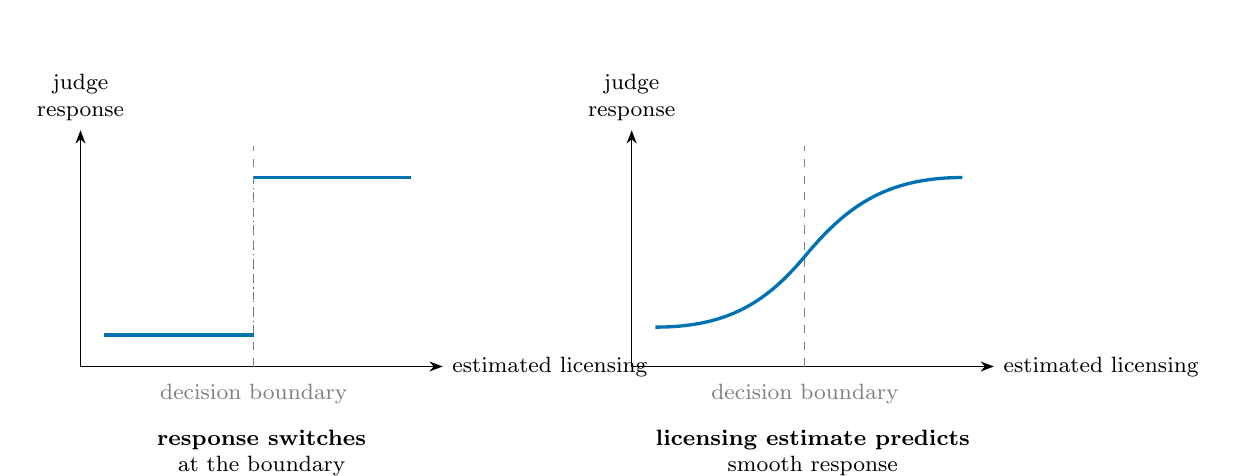
\begin{tikzpicture}[font=\small, >=Stealth]
\begin{scope}
  \draw[->] (0,0) -- (4.6,0) node[right, font=\footnotesize] {estimated licensing};
  \draw[->] (0,0) -- (0,3) node[above, font=\footnotesize, align=center] {judge\\ response};
  \draw[dashed, gray] (2.2,0) -- (2.2,2.8);
  \node[font=\footnotesize, gray] at (2.2,-0.35) {decision boundary};
  \draw[very thick, lsMidBlue] (0.3,0.4) -- (2.2,0.4);
  \draw[very thick, lsMidBlue] (2.2,2.4) -- (4.2,2.4);
  \draw[dotted, lsMidBlue] (2.2,0.4) -- (2.2,2.4);
  \node[font=\footnotesize, align=center] at (2.3,-1.1) {\textbf{response switches}\\ at the boundary};
\end{scope}
\begin{scope}[xshift=7cm]
  \draw[->] (0,0) -- (4.6,0) node[right, font=\footnotesize] {estimated licensing};
  \draw[->] (0,0) -- (0,3) node[above, font=\footnotesize, align=center] {judge\\ response};
  \draw[dashed, gray] (2.2,0) -- (2.2,2.8);
  \node[font=\footnotesize, gray] at (2.2,-0.35) {decision boundary};
  \draw[very thick, lsMidBlue] (0.3,0.5)
    .. controls (1.2,0.5) and (1.7,0.8) .. (2.2,1.4)
    .. controls (2.7,2.0) and (3.2,2.4) .. (4.2,2.4);
  \node[font=\footnotesize, align=center] at (2.3,-1.1) {\textbf{licensing estimate predicts}\\ smooth response};
\end{scope}
\end{tikzpicture}
\caption{The decision-layer discontinuity check. If asymmetric losses induce a
response switch, a judge's treatment of a form should change abruptly as the
judge's estimated licensing crosses the practical boundary (left); if the
read-out tracks that estimate continuously, treatment should vary smoothly
through it (right). A regression-discontinuity design on multinomial hearer
responses targets this decision layer, not the constitutive status state itself.}
\label{fig:rd-test}
\end{figure}

\clearpage
\section{Conclusion}

Grammaticality, de-idealized, isn't one fact about an ideal speaker. It's a
conditioned profile: whether some assembly covers a form and its intended value,
whether its operator contributions unify, whether its obligatory contrasts are
supplied, and whether the relevant population licenses its constructions. A
speaker's evidence about that profile and the resulting feelings of anomaly and
confidence are separate objects. So are genuine differences among speakers and
mere uncertainty about the population mean.

The point of the profile is projection. Weakly evidenced forms should respond
differently to framing and exposure from forms repeatedly defeated in genuine
opportunities; licensed but processing-heavy forms should improve without a
change in licensing; moribund contrasts should lose evidential support before
their categorical treatment disappears; and operator errors should draw a
different repair profile from value-intact constructional errors. These claims
are informative only if situations, niches, alternatives, and target
projections are fixed before the outcomes are inspected.

The population dynamics establish the possibility of separated licensing
regimes under independently motivated adoption and retention conditions.
Evidence updating alone is insufficient. Repair is a candidate maintainer or
controller, not one by definition; maintenance requires transmission evidence,
and control requires a deviation-sensitive intervention that restores the
threatened relation. A
history-dependent loss-and-recovery pattern is likewise predicted only where
two stable regimes and their external controls have first been established.

The resulting account is less simple than a single grammaticality score, but its recurring
distinctions handle cases that otherwise demand unrelated explanations. Their
economy has to be earned empirically: estimate licensing from converging
non-rating indicators, normalize production by independently specified
opportunities, and let the projections fail when their indicators are wrong.
De-idealizing grammaticality thereby replaces a tractable fiction with a
category that answers to evidence and predicts which rejections soften, which
forms transmit, and which absences hold.

\newpage
\appendix

\section{Turkish vowel harmony and operator-exponent realization}
\label{app:turkish-harmony}

Turkish illustrates a sharp distinction between \term{lexical} disharmony inside stems and
\term{allomorphic} harmony on inflectional suffixes.%
\footnote{See \autocite{Sezer1981,KabakVogel2001} for discussion of the phonology and \autocite{Arik2015} for experimental evidence on native judgments.}
OVMG treats suffixal harmony as operator-exponent licensing and stem disharmony
as lexical licensing. Vowel backness isn't a public-update value; plural and
past are. In Turkish, the exponents of those operators have to satisfy suffixal
harmony.

\noindent\textsc{Stem-internal vowels: disharmony tolerated.} Loanwords such as
\mention{doktor} `doctor' violate backness harmony, but are fully acceptable;
speakers store the form, and the community licenses it consistently.

\ea \label{ex:doktor}
\gll \mention{doktor} \\
     doctor\\
\glt `doctor' (disharmonic stem, grammatical)
\z
Because the word contains no malformed operator exponent, a stored construction
covers it, the relevant operators unify, and the word is licensed.

Such forms can begin with narrow licensing in borrowing, quotation, or bilingual
situations whose participants share access to the foreign expression. Repeated
adoption and retention can extend an item beyond that niche until speakers store
it as an ordinary lexeme. The result is item-specific licensing of
\mention{doktor}. Stem disharmony doesn't become a productive pattern, and the
suffixal harmony requirements remain unchanged.

\noindent\textsc{Suffixal harmony: operator-exponent licensing.} Inflectional morphemes are lexicalized with an underspecified vowel; the licensed allomorph copies stem backness and, for some suffixes, rounding. Using the \enquote{wrong} vowel doesn't make the intended value unrecoverable: speakers can identify \mention{-ler} as a plural exponent and \mention{-du} as a past exponent. What fails is licensing of that exponent choice in a dense operator-exponent niche.

\ea  \label{ex:kitap-pl}
\ea[]{\gll \mention{kitap-lar}\\
          book-\textsc{pl.back}\\
      \glt `books' (harmonic, grammatical)}
\ex[*]{\gll \mention{kitap-ler}\\
          book-\textsc{pl.front}\\
      \glt intended `books' (suffix harmony violation)}
\z
\z

\ea \label{ex:gul-past}
\ea[]{\gll \mention{gül-dü}\\
          laugh-\textsc{pst.front.round}\\
      \glt `s/he laughed' (harmonic, grammatical)}
\ex[*]{\gll \mention{gül-du}\\
          laugh-\textsc{pst.back.round}\\
      \glt intended `s/he laughed' (suffix harmony violation)}
\z
\z

\noindent\textsc{OVMG account.} For the ill-formed \ungram{\mention{kitap-ler}} and \ungram{\mention{gül-du}}:

\begin{itemize}
\item The plural and past constructions are securely licensed at the population
  level. The mismatched exponent choice isn't licensed.
\item The mismatched allomorph is still identifiable as an intended exponent,
  so the token is covered by a candidate operator-exponent assembly. But its
  exponent-choice node is almost universally excluded by overwhelming
  preemption from harmonic suffix choices across the many plural and past
  opportunities. The result is concentrated non-licensing and high confidence,
  not empty coverage.
\end{itemize}

Repeated suffix opportunities support the same allomorphic choice, yielding
confident categorical rejection. This keeps suffix-harmony errors apart from
word salad. \ungram{\mention{Can the
have running}} lacks a covering assembly; \ungram{\mention{kitap-ler}} has a
recoverable intended value and an identifiable exponent, but the exponent
choice is almost universally excluded. By contrast, \mention{doktor} in
(\ref{ex:doktor}) is
covered by its own stored node: stem disharmony violates no operator-exponent
licensing condition, so the word remains licensed and the disharmony registers
only as a phonological cost in the subjective read-out
(\S\ref{sec:feeling-new}).

\noindent\textsc{Localized exceptions.} Some derivational suffixes (e.g.~\mention{-imsi} `-ish') are lexically
marked \enquote{disharmonic}. Speakers store them, and community licensing
remains consistent: no
exponent condition is violated, so the form remains licensed despite vowel
mismatch. Clitic
boundaries that start a fresh harmony cycle \autocite{KabakVogel2001} are
handled the same way: they satisfy the operator-exponent requirement and leave
harmony to phonology alone.

Turkish suffix-harmony errors are grammaticality failures in a precise sense:
they don't mis-set a public-update contrast themselves, but they choose an
unlicensed exponent for a closed inflectional operator in a dense niche. Stem
disharmony lowers phonological well-formedness and affects only the subjective
cost vector. A counterexample to the operator-specific response claim would be
a matched phonological contrast with no operator-exponent role that produced the
same update-confusion and update-oriented repair profile.


\section*{Acknowledgements}
Thanks to Peter Evans, Geoff Pullum, Muhammad Ali Khalidi, Ryan Nefdt, Irene Kosmas, and Mostafa Hasrati for comments and suggestions. I'd like to thank Jamie Ramsden for discussions that sharpened the treatment of situational licensing, and Henri Kauhanen for reviewing the formalization.

\clearpage
\begin{sloppypar}
\printbibliography[title=References]
\end{sloppypar}


\end{document}
